\section{Introduction}
It is estimated that 13.7 billion Danish kroner is lost each year on Danish vehicles stopping at traffic ligts.\cite{Vejdir}
It is a well known fact that a vehicle driving at a constant velocity use less fuel than an accelerating vehicle due to the physical laws of motion.
In order to save fuel, one should therefore try to drive with a constant speed.
It is esimated that a total of 1.8 bilion Danish kroner is lost on fuel each year and the socio-economic cost of time lost in traffic lights in Denmark is estimated to 9.5 billion Danish kroner. 
Lost time is defined as how much the driver is delayed by decelerating and stopping for a red light and accelerate again.

Traffic lights hinders the flow of traffic as it blocks vehicles arriving from one direction in order to allow other vehicles to drive through the intersection.
Normally, a driver will only be able to guess when the light is going to change based on local knowledge of the area. 
Looking at Figure \ref{fig:Introduction:network} vehicle $\veh_2$ is approacing the intersection.
Now assume that vehicle $\veh_2$ knows the distance $\dist_3$ where he has to stop for the traffic light. 
Furthermore assume that vehicle $\veh_2$ knows that in $4$ seconds the traffic light will change to green. 
Then it is posible to calculate at which speed $\veh_2$ should drive such that it will drive the distance $\dist_3$ in $4$ seconds. 
Now by the time the vehicle reaches the intersection the signal will have changed and the vehicle can maintain its speed driving through the intersection.
\begin{figure}[htb]
\centering
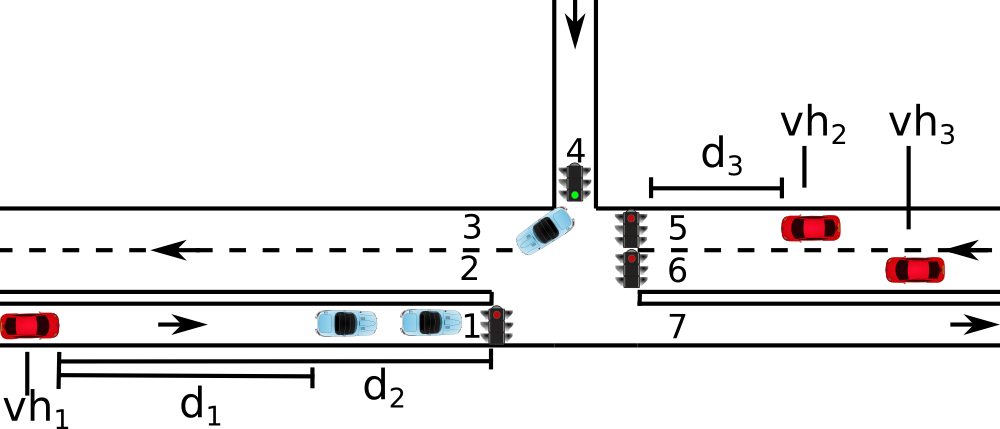
\includegraphics[width=0.45\textwidth]{../images/introNetwork.png}
\caption{Example network}
\label{fig:Introduction:network}
\end{figure}

Road authorities try to design traffic lights such that the flow of traffic is maximised in all directions.
This is very difficult, especially in junctions with changing traffic density through out the day.
Two main techniques are used for traffic lights: pretimed traffic controllers, where the signals loop between red, yellow and green in a predefined pattern; and traffic actuated controllers, where approacing vehicles are detected by road-side detectors such that the signals can be adjusted to the current traffic flow \cite{Vejdir}.
The cost of upgrading a traffic light with detectors is 200.000-300.000 Danish kroner\cite{Vejdir}.

We focus on investigating whether it is possible to reduce the fuel consumption at pretimed traffic lights and increase overall traffic flow by matching driving speed to traffic lights. 
We investigate this through simulations based on real-world maps, traffic data and traffic light programs.
Simulations are much cheaper, faster and safer than large-scale field studies. 
We use the traffic simulator SUMO (Simulation of Urban Mobility)\cite{sumo} which is a full scall microscopic traffic simulator.

The main contributions of this work are:
\begin{enumerate*}
\item The system does not require communicaiton between vehicles. This reduces communication cost and the system can be used independent of the penetration rate.
\item Users of the system achieve a considerable reduction in fuel consumption. The reduction is almost independent on the number of users and even non-users see a slight fuel reduction with higher penetration rates.
\item The system helps drivers avoid stopping at traffic lights, which improves overall traffic flow, especially with higher congestion.
\item \tech is evaluated through simulations with a realistic setting, and comparable results are compared with data from GPS trajectories.
\end{enumerate*}

\tech has the potential to be implemented on an every day smartphone. 
Many already have a smartphone that has GPS systems, internet access, maps and enough processing power and memory.
The advised speed can accompany the build in GPS system as a minimalistic graphical overlay, which will make it readily available for the user.

The remainder of the paper is organised as follows: 
We describe the related work in Section~\ref{sec:RelatedWork} and the model in Section~\ref{sec:Model}. 
In Section~\ref{sec:Math}, we detail the proposed techinique by going through the algorithm.
Section~\ref{sec:UseCase} is about the use case that we test the proposed technique on, and the results of these tests are evaluated in Section~\ref{sec:Test}. 
We conclude the findings in Section~\ref{sec:Conclusion}.




